\documentclass[msthesis.tex]{subfiles}

\begin{document}
\chapter{Background}
Non-invasive neuroimaging techniques have become indispensable tools to understand cognitive processes and neurological disease pathology. \gls{dMRI} is a new type of imaging modality often used to produce highly detailed anatomical images. It is of high utility when required to look at soft tissues such as those in the nervous system. With the help of white matter studies, more information about connectivity and extraction can be seen.

Classification based on Neuroimaging techniques is an intricate task. It suffers from the curse of dimensionality and the results need to be interpretable for the classifiers to be actually used in either clinical practice or Neuroscience research. Even though machine learning is readily applied in this field of study it suffers from the lack of interpretability of predictions. Using graph based techniques along with feature selection methods can help establish Neurobiological correspondence of the basis of classification made by the classifier.  

\iffalse
From neurobiology, it is known that neurons are the fundamental units of the brain and the nervous system. Each neuron contains the main the cell body, the axons (encoated with a myelin sheath) and dendrites (the strands that connect the end of one neuron to the starting of the second neuron - presynaptic and postsynaptic terminal), the synapse as the junction between the first neuron and the next one. 

(INSERT THE PICTURE OF A NEURON)

The axons, often termed as white matter tracts due to their myelination are on an average 1m long and run along the brain. These form the basis for the getting the structural brain connectivity, one connection between different regions of the brain is recognized as one axonal streamlines.
\fi
\section{Magnetic Resonance Imaging}
\gls{MRI} is a non-invasive imaging technology that can produce 3-dimensional detailed anatomical images \citep{mcrobbie_moore_graves_prince_2006}. This technique is based on the \gls{NMR} Imaging principle. \gls{NMR} a physical phenomenon in which nuclei respond to a combination of a constant and weak oscillating magnetic field by producing a signal at the resonant frequency of the nucleus. The difference between the magnetic properties of different tissue types subjected to an external magnetic field is used to generate images. Such electromagnetic properties are used to form images since our body is 65\% water ($H_2O$), has a dipole moment and the hydrogen nuclei act like little magnets due to the fact that hydrogen nuclei have an odd number of protons and non-zero net spin. 

In normal conditions (\autoref{mriphysics}.a), i.e. in the absence of an external magnetic field the spins of the hydrogen nuclei are randomly oriented and cancel out each other when observed as an ensemble. Once the external field is applied, the hydrogen nuclei exhibit their paramagnetic nature and gain a net magnetization in the direction of the external magnetic field and transverse magnetization as the one perpendicular to it. This can be represented using the equation
\begin{equation}
       \Vec{M_o} = \mu \Vec{B_0}
\end{equation}
where M is the magnetization, $\mu$ is the magnetic permeability or the inertia of a material to get magnetized and $B_0$ is the external magnetic field. According \autoref{mriphysics}.a, it can be seen that the direction of $B_0$ defines the coordinate system for the experiment. The transverse plane is defined as the plane perpendicular to the direction of $B_0$ whereas, the longitudinal magnetization is termed as the magnetization experienced in the direction of the static magnetic field. In the presence of the external static magnetic field the individual nuclei are precessing (rotating around their axis) with a frequency known as the Larmour frequency, which can be expressed by the equation
\begin{equation}
    \omega_0 = \gamma B_0
    \label{larmour}
\end{equation}
where $\omega_o$ represents the frequency, $\gamma$ represents the gyromagnetic ration and $B_0$ the exernal field.
\begin{figure}
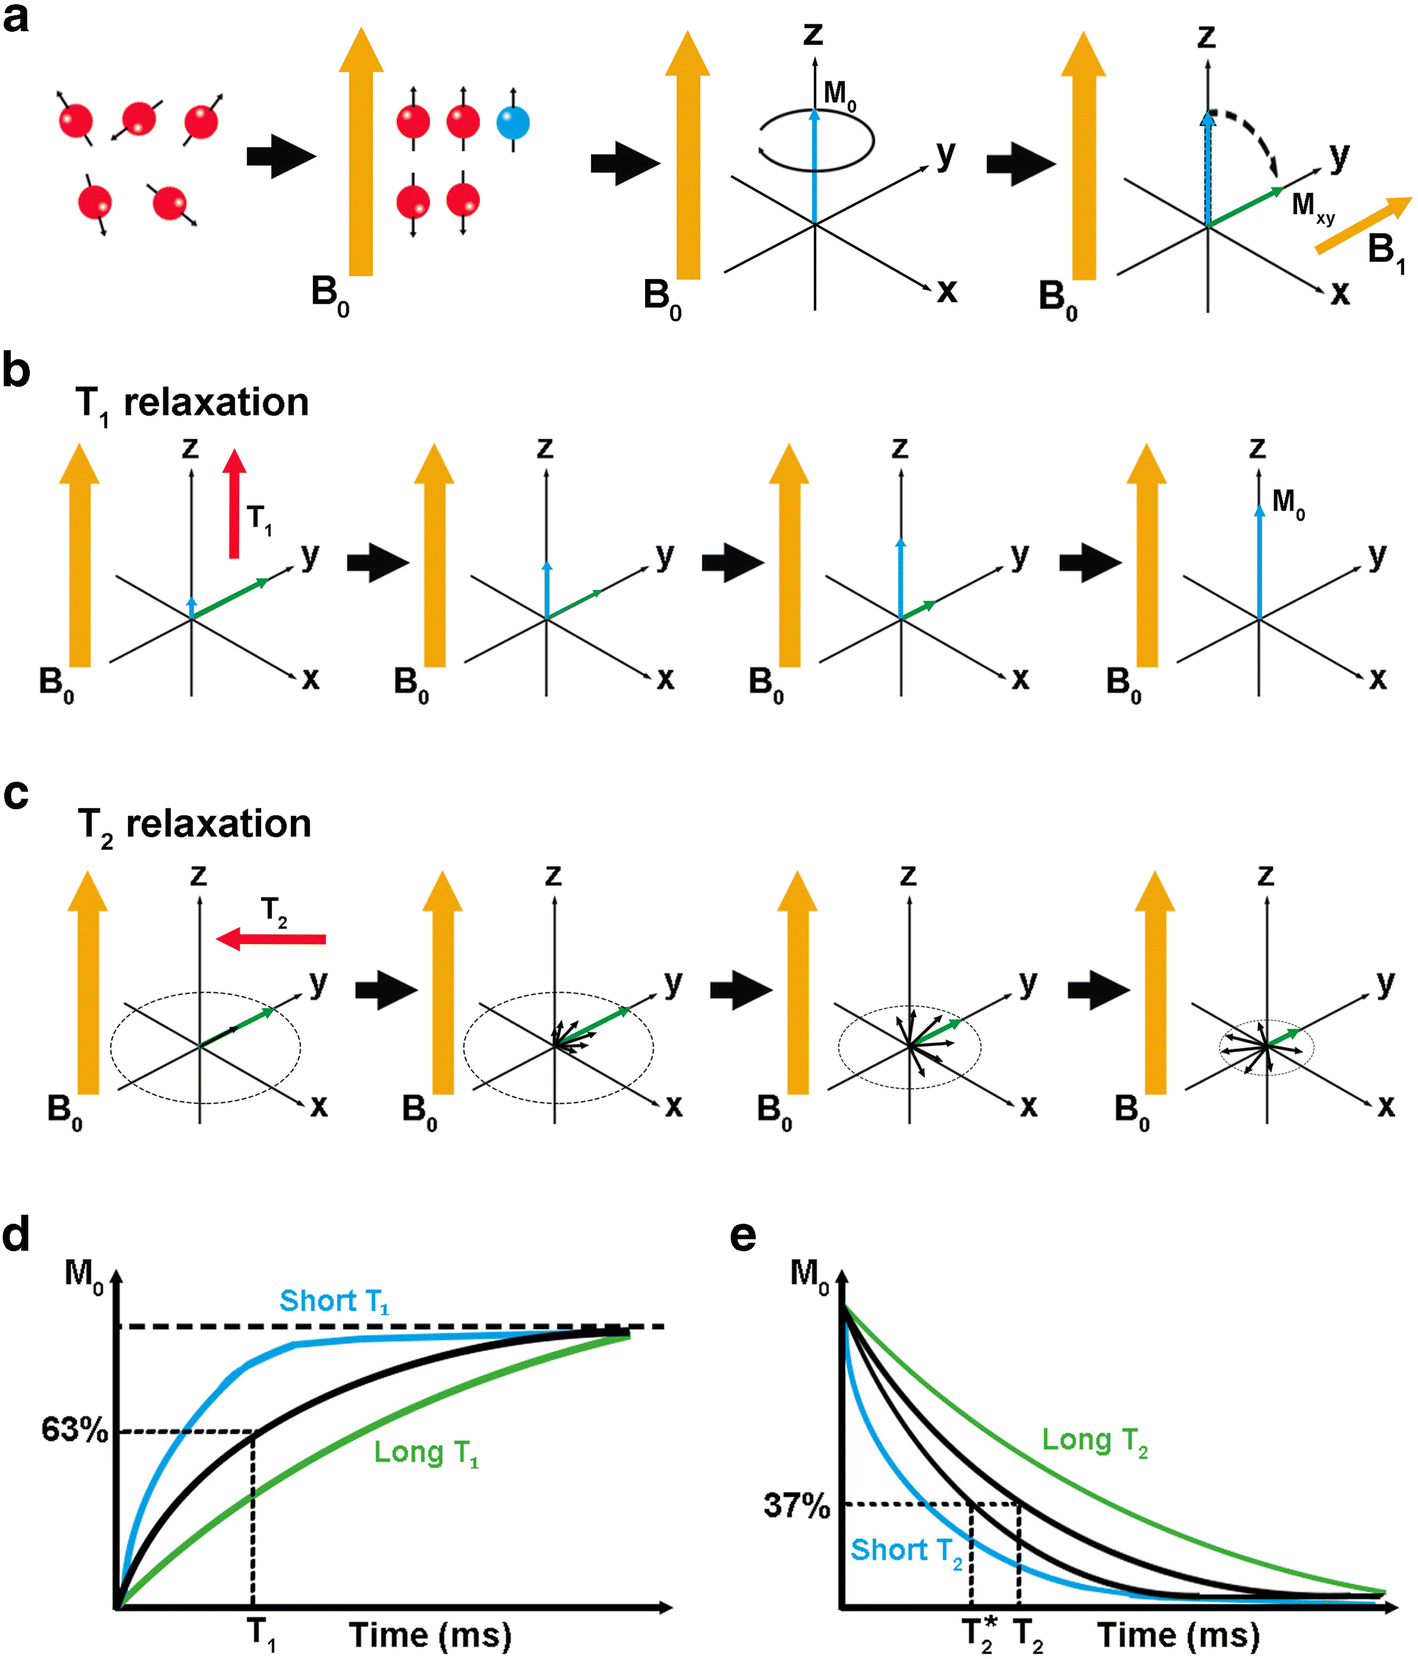
\includegraphics[width=0.847\textwidth]{images/mri1.png}
\caption{figure from \cite{Mastrogiacomo2019}. (a) At first the magnetic moments of the individual nuclei are oriented randomly and cancel out each other, in the presence of an external field $B_0$ they gain a net magnetization, with the presence of the external RF pulse the phase of the net magnetization is changed and magnetic resonance is said to occur. (b) Describes process of T1 relaxation in which the net magnetization starts to align along the static magnetic field $B_0$. (c) Describes T2 relaxation or the dephasing of magnetization in the transverse plane. (d) Illustrates that the value of the T1 constant is the time required to achieve 63\% of the longitudinal magnetization. (e) The time constant T2 is the time required for the magnetization to fall to 1/e of its value. In (d) and (e) the blue lines represent tissues containing fat while the green lines represent fluids such as \gls{CSF}}
\label{mriphysics}
\end{figure}

When a radio wave is added to the static field using a radio frequency coil (RF coil) at the Larmour frequency (\autoref{larmour}), termed as $B_1$ in \autoref{mriphysics}.a, the direction of the magnetization vector gets altered i.e. ‘flipped’ or ‘tipped’ out of alignment with $B_0$ towards $B_1$ with the angle of rotation being termed as the flip angle. The RF pulse causes exerts torque. Mathematically, the torque can be expressed as
\begin{equation}
    \Vec{\tau} = \Vec{m} \times \Vec{B_1}
\end{equation}
where $\Vec{m}$ represents the magnetic moment and the $ \Vec{B_1}$ is the applied magnetic field.The flipping does not bring all the spins in phase with each other but the net magnetization gets flipped ($M_{xy}$) onto the transverse plane. The magnetization $M_{xy}$ then precesses in this plane.

The net magnetization does not precess until an external force disturbs its equilibrium position of alignment with the static magnetic field. Thus, when the magnetization precesses, magnetic resonance is said to occur. The magnetization has an effect in which the frequency is proportional to the applied static magnetic field.

After this, the RF pulse is switched off which causes the tissue molecules to return to their original state and is termed as the relaxation phase. The relaxation is due to the release of electromagnetic energy into the environment to attain thermal equilibrium. This release of electromagnetic energy is what forms the signal for the receiver coil, \cite{PhysRev.70.460} introduced two time constants to measure the relaxation phase, T1 and T2.

The constant T1 measures the growth of the longitudinal component ($M_z$, \autoref{mriphysics}.b) with T1 relaxation being termed as the process by which the net magnetization aligns itself with the direction of the original magnetic field. The T2 constant measures the decay of the transverse component of the magnetization (\autoref{mriphysics}.c). The value of T2 reflects the time required for the magentization to fall to $\frac{1}{e}$ or 37\% of its original value, reflected in \autoref{mriphysics}.e. Since there can be imhomogneties inside the \gls{MRI} scanner, another constant $T2^*$ is measured as the T2 time observed while taking the recording.
During the resonance phenomena, the magnetization has components in different directions which can be expressed in terms of the time constants and current time
\begin{equation}
    M_x(t) = M_o e^{\frac{−t}{T2}} \sin{ \omega t}
    \label{mx}
\end{equation}
\begin{equation}
    M_y(t) = M_o e^{\frac{-t}{T2}} \cos{\omega {t}}
    \label{my}
\end{equation}
\begin{equation}
    M_z(t) = M_o (1 − e^{{\frac{−t}{T1}}})
    \label{mz}
\end{equation}
Where $M_x$ ,$M_y$, $M_z$ are the magnetizations along the x,y and z directions and $M_0$ is the magnetization induced by the applied static magnetic field $B_0$. From the \autoref{mz} it is clear that the T1 constant measure the time required to gain the original magnetization, i.e. when $t=T1$
$M_z = M_0$ and when $t=T2$, $M_{xy} = \frac{M_0}{\cos{\omega T2}}$


T1 weighting is generated on the basis of controlling the \gls{TR} in a sequence. The \gls{TR} is defined as the time taken between successive excitations of the same region. Using a small \gls{TR} causes the net magntizations aligned along the fields to not fully recover. Different brain tissues have different T1 values. Short T1 times are seen in fat molecules because of their complex structure. The intricacies of saturated molecules lead to flexions and roations which might occur at the Larmour frequency. This makes it easier for the magnetization to return to the initial state (longitudinal orientation). Longer T1 times are observed in comparatively freely diffusing mediums such as \gls{CSF}. Such fluids appear dark on T1-weighted images due to longer T1 times while fat molecules appear bright with the same diffusion weighting.

Similar to generation of a T1 image on the basis of \gls{TR}, T2 weighting of an image is generated on the basis of \gls{TE}. The \gls{TE} measures time between excitation and signal measurement. A well adjusted, long TE gives rise to contrast of signals from different images. Fat molecules appear lighter on T2-weighted images due to short T2 time while the \gls{CSF} appears bright since it has long T2 times.


\subsection{Image formation}

An \gls{MRI} scan needs to represent the 3D nature of the body part under study. Inside an \gls{MRI} scanner, the gradient coils are used to alter the magnetic field along the different spatial directions. This ensures that different slices of the subject’s body resonate at different frequencies. The signal from all the slices is then received by receiver coils that detect only the transverse magnetization. For example in neuroimaging, this signal needs spatial encoding since information about the millions of voxels in the brain.

\begin{figure}
    \centering
    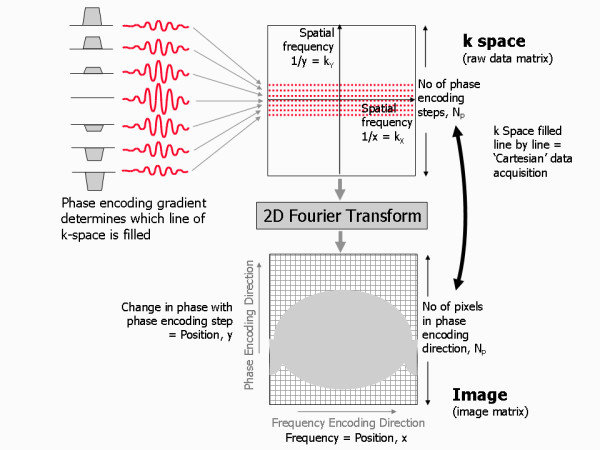
\includegraphics[width=\textwidth]{images/img_reconstruction.jpg}
    \caption{Image from \cite{MRIrecon} summarising the reconstruction of an encoded \gls{MRI} signal in 2D, after a slice has been selected using the gradient $G_z$. The phase is encoded along the y direction. Each phase encoding step is used to populate the k-space. The number of such steps determine the number of pixels in the y-direction. The frequency is encoded along the x direction. The relationship between the k-space points and the points in reconstructed image space is such that $k_x =1/x$ and $k_y= 1/y$. Each line parallel to the $k_x$ axis corresponds to a separate MRI signal. At the same time each line parallel to the $k_y$ axis corresponds to the amplitude and duration of the phase encoding direction at each phase encoding step.}
    \label{fig:mri_img}
\end{figure}

It is known that in order to form the 3D image the magnetic gradients are applied in the x,y,z directions. This formalism results in each voxel possessing a different Larmour frequency and the phenomenon can be termed as spatial encoding. 
\begin{equation}
        \label{eq:larmour_grad}
          \omega = \gamma(B_0 + G(x, y, z))
     \end{equation}
       
According to \autoref{eq:larmour_grad}, it is prominent that there is a direct relation between the gradient field and the Larmour frequency. Usually the gradient for the slice selection is applied along the z-direction. For better understanding a simpler case of 2D image reconstruction has been explained in the \autoref{fig:mri_img} where the phase encoding gradients are applied in a direction perpendicular to the frequency encoding gradients.

The \gls{RF1} coils in the \gls{MRI} scanner detects a signal containing a mixture of frequencies specific for each slice and each phase encoding step. The distribution of frequencies is determined using a Fourier transform. This distribution is then used to fill what is called as the k-space. The 2D k-space in \autoref{fig:mri_img} is used to elucidate the components of the frequency. The intensity of a point in the space represents the contribution of the frequency $(k_x,k_y)$ in the signal. For each combination of $(k_x, k_y)$ in the k-space the scanner camera takes only one picture (one filter per voxel) and then estimates the actual intensities at different locations using an inverse Fourier transform. There is a one-to-one correspondence of the pixel in the k-space to the image space. Every pixel in the 2D k-space image maps to only one pixel in the reconstructed 2D image. However, it is not necessary that the locations in both the images are exactly the same. This mapping using a Fourier transform is then extrapolated in 3D in order to obtain the image of the whole organ such as the brain. Any weighting such as T1 or T2 can be given in order to generate the image after the transformation has taken place.

Another important concept for image formation is that of \gls{FOV}. It refers to the distance over which an \gls{MRI} signal is acquired or displayed. The defined \gls{FOV} determines the pixel width (determined by the phase encoding y-direction in \autoref{fig:mri_img}) given by $\Delta k = 1/FOV$. 

\subsection{Diffusion MRI}

\gls{dMRI} is an \textit{in-vivo}, non-invasive imaging modality that used to create high-resolution structural images of biological tissues. It measures the non-homogeneity of water diffusion in tissues to probe their microstructure \citep{ghosh2015survey}. One of the most important applications of \gls{dMRI} is to map the white-matter fiber tracts in the brain. As compared to other \gls{MRI} techniques such as \gls{fMRI} it does not suffer from an issue of low resolution and low signal-to-noise ratio \citep{wong2016}. 

`Diffusion' is defined as the net movement of a substance from a region of higher concentration to a region of lower concentration. In a homogeneous medium, the diffusion of water molecules is isotropic, i.e. the molecules can move in any direction with equal probability. They exhibit random walk behavior which is explained by Brownian motion \citep{Brogioli_2000}.

The environment inside a biological tissue is complex and the diffusion of water molecules becomes anisotropic due to the hindrances imposed by cellular membranes. Water molecules in the extracellular environment hence experience relatively free diffusion and the ones in the intra-cellular environment experience restricted diffusion \citep{toennies2017guide}. This diffusion anisotropy is encoded into the MRI signal using spatial and temporal variation (gradients) in the magnetic field. This means that the alignment of the molecules is influenced by the diffusion direction. The \gls{MRI} signal is said to be `Diffusion Weighted' due to the signal attenuation introduced by the magnetic field gradients. 


\subsubsection{Diffusion Weighted Imaging}
\begin{figure}
    \centering
    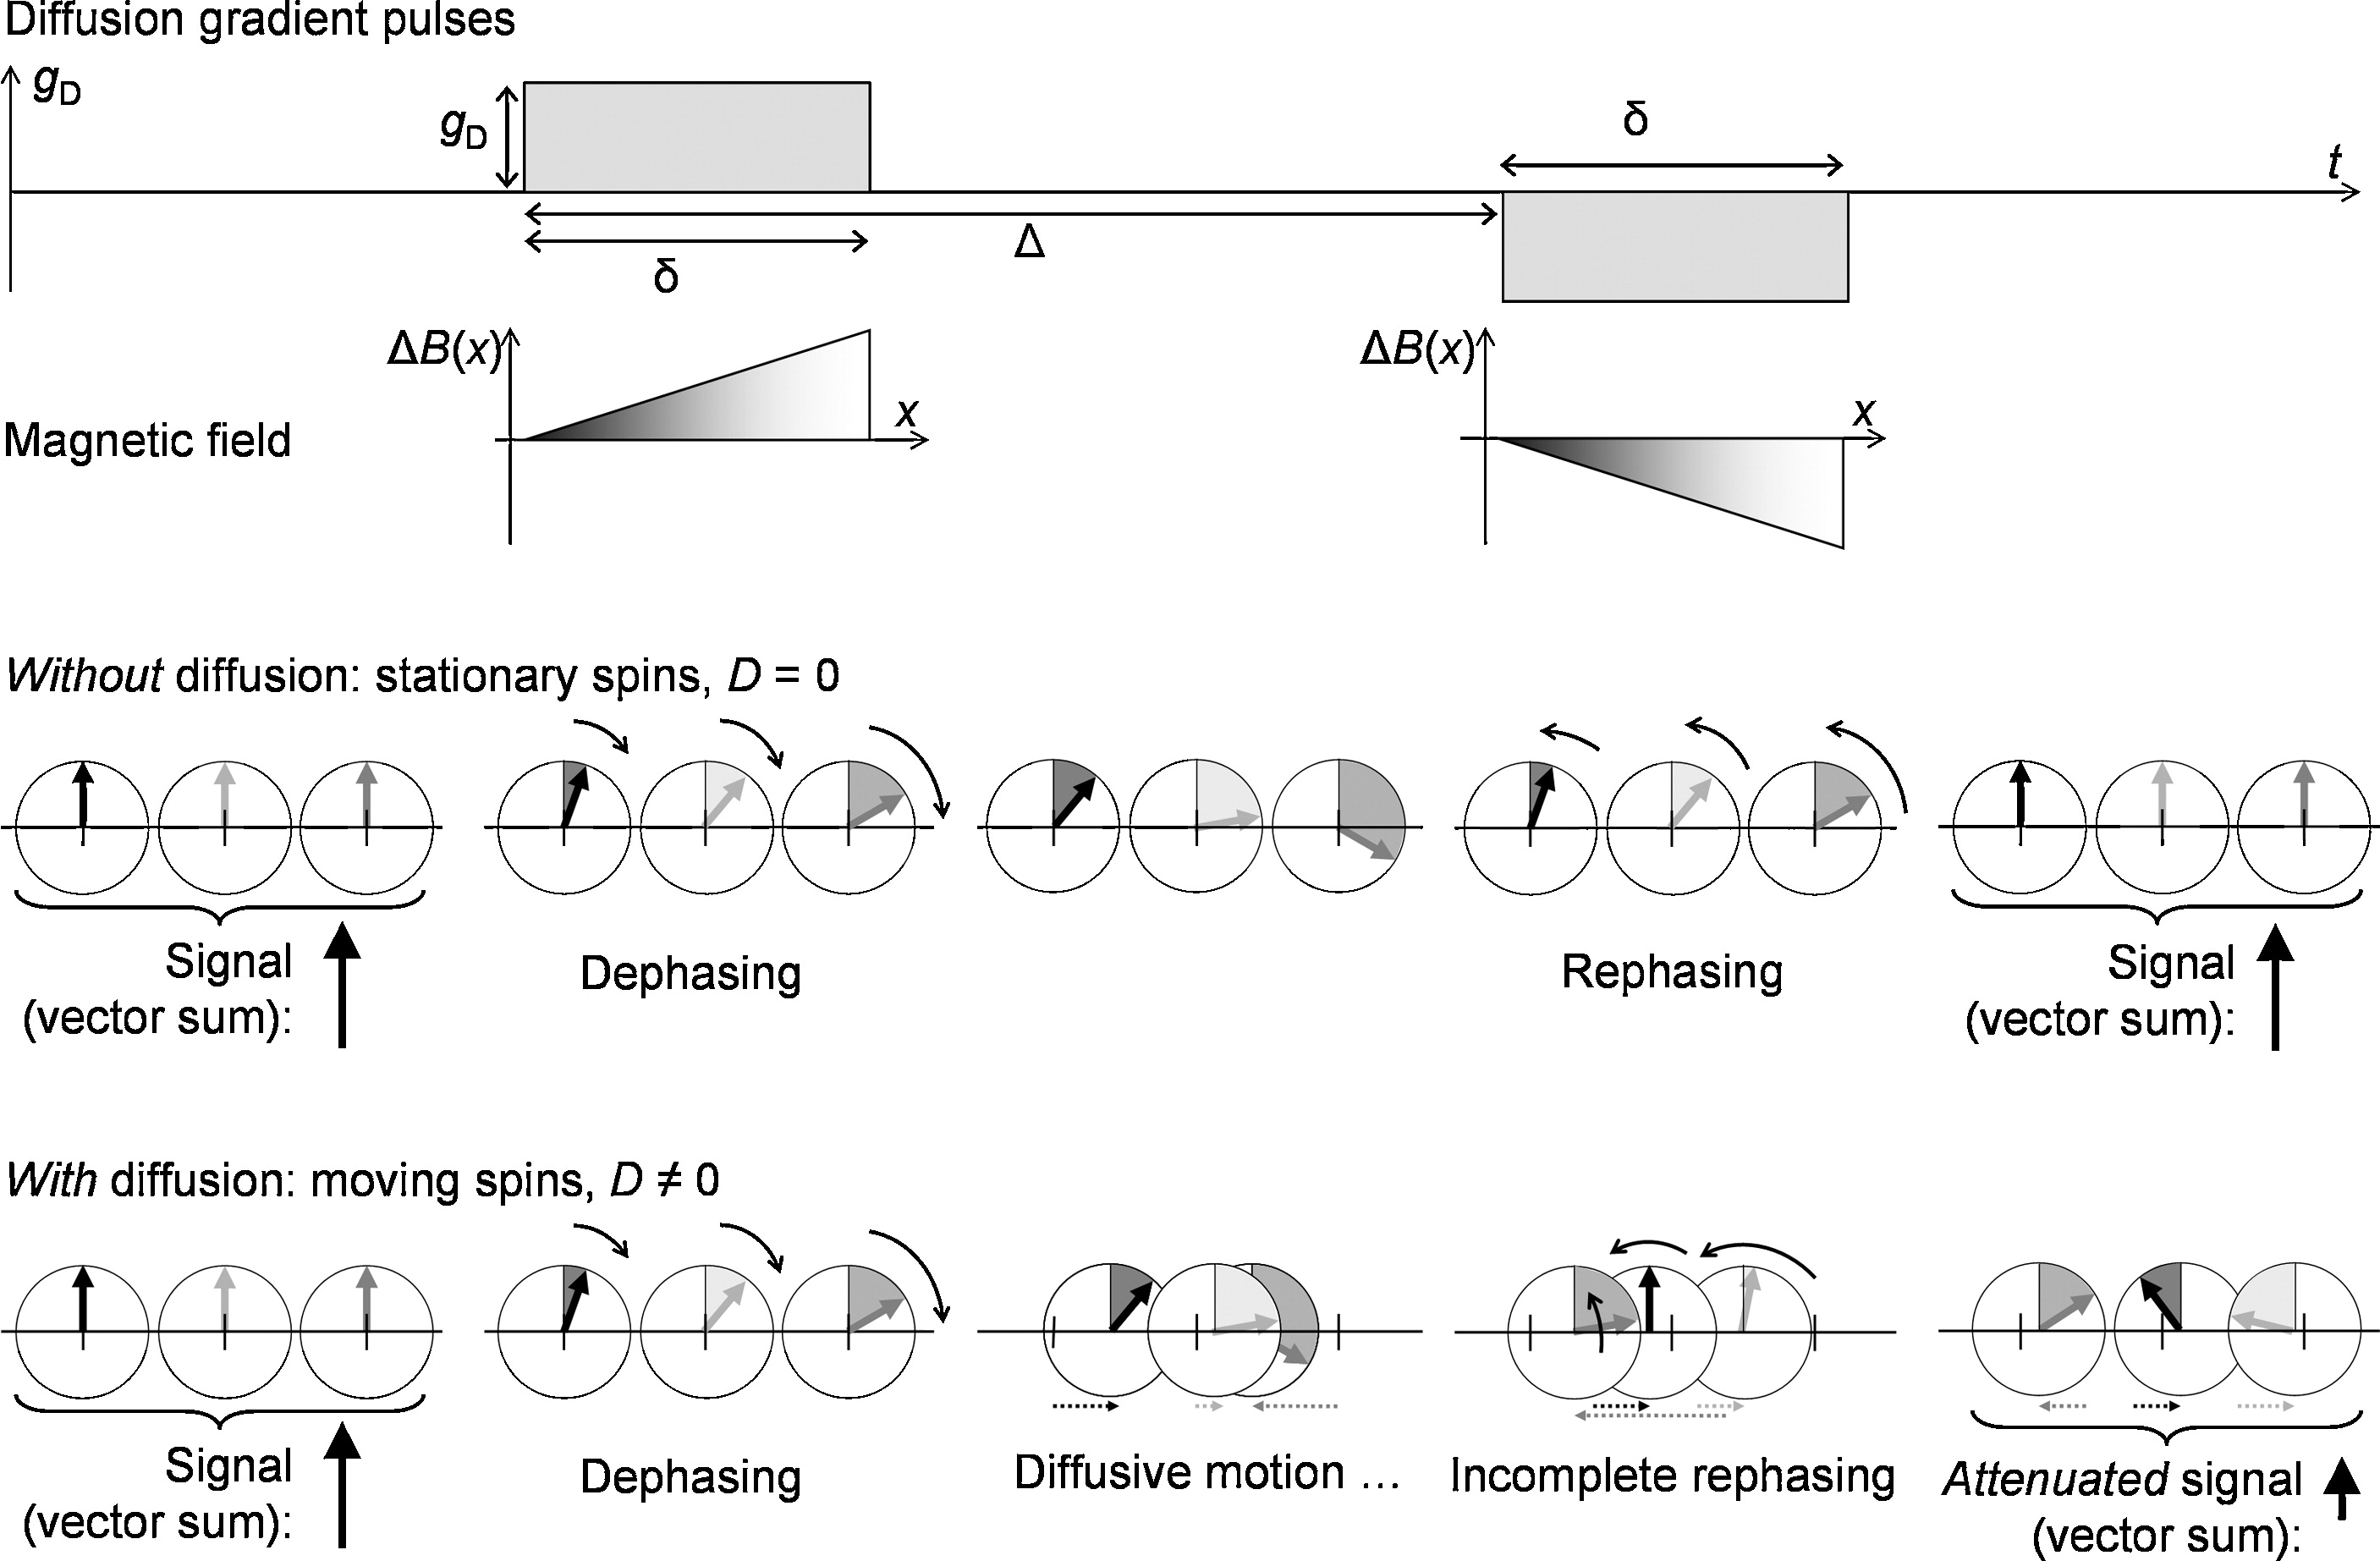
\includegraphics[width=\textwidth]{images/diffusionmri.jpg}
    \caption{Image from \cite{technical_aspects_dmri} elucidating the technical aspects of Diffusion Weighted MRI. The RF pulse causes a phase change of the net magnetization. Introducing the diffusion gradient adds spatial dependence of phase shift on the individual magnetic moments. The molecules that have restricted diffusion do not experience the effect of the diffusion gradient, any phase change from the first gradient is reversed by the second. They tend to relax to their equilibrium state. However, molecules that undergo free diffusion experience the effects of the diffusion gradients introduced by the second RF pulse (180 degrees) and hence will undergo a total phase shift dependent on the spatial location. This shift is manifested in terms of signal attenuation. The degree of signal attenuation depends on multiple factors as shown in \autoref{eq:Stetjskal}.}
    \label{fig:diffmri}
\end{figure}
\label{sec:DWI}
In this type of Diffusion imaging, the intensity of each voxel represents the rate of water diffusion in a cubic region. Diffusion weighting is applied in order to generate contrasts based on the presumption that diffusion varies with pathology i.e. differences in diffusion can also highlight differences in structure and function \citep{Taylor_1985}. 

One of the most popular ways to give images Diffusion weighting is through using \gls{SE} T2 weighted sequences with two symmetric gradients on each side of the 180 degree refocusing pulse. This is based on the \gls{PGSE} technique developed by \cite{stejskal1965spin}. PGSE resulted in improved sensitivity to diffusion in comparison to the steady state gradients used previously. \cite{stejskal1965spin} solved the Bloch-Torrey \citep{bloch1946nuclear} partial differential equations for a symmetric pair of pulsed gradients and obtained the well-known Stejskal-Tanner formula
\begin{equation}
\label{eq:Stetjskal}
S = S_0 \exp^{-bD}
\end{equation}
$S_0$ represents the original signal strength, $S$ is the signal strength in a pulse sequence with the presence of diffusion gradients ($g_D$) and $D$ represents the diffusion coefficient. The the attenuation of the \gls{dMRI} signal by the diffusion gradients is represented in \autoref{fig:diffmri}. The application of the diffusion gradient results in a spatial encoding as the Larmour frequency becomes dependent on the net magnetic field (\autoref{eq:larmour_grad}. In \autoref{fig:diffmri}, it is evident that the Diffusion gradients are magnetic field gradients along the $x$ direction. 

Here $\Delta B_(x) = g_D x$ which makes the Larmour frequency spatially dependent $\Delta \omega = \gamma \Delta B_(x)$ or $\Delta \omega = \gamma g_D x$. There is a phase shift introduced after the gradient pulse of time duration $\delta$. The the phase shift is also dependent on the x position due to the spatial dependence of $\Delta w(x)$ , the phase shift is $\Delta \phi (x) = \Delta w \delta = \gamma g_D x \delta$. This spatial dependence of the phase shift makes spins at different positions along the gradient axis `dephased' after the application of the gradient pulse. When the negative gradient is applied, the process of rephasing occurs. The dephasing and rephasing mechanisms result in the diffusion weighting of the image. Without any diffusion stationary spins would align along their equilibrium position (cancelling effect of the two opposing diffusion gradients) while with diffusion weighting there is a signal attenuation explained by \autoref{eq:Stetjskal}. 

The b value of the diffusion weighted sequence mentioned in \autoref{eq:Stetjskal} is defined in the units of $s/mm^2$ as
\begin{equation}
    b = (\gamma g_D \delta)^2 (\Delta - \frac{\delta}{3})
\end{equation}
In order to obtain the numerical value of b, long and strong gradients are required. The diffusion gradients $g_D$, time of pulse $\delta$ and time interval $\Delta$ are often adjusted to adjust the b values. Higher b values leads to lower signal in the areas of high diffusion and increases the contrast between tissues that have different diffusion coefficients. The b values often need to be adjusted to obtain an optimal \gls{SNR}


\subsubsection{Diffusion Tensor Model}
\gls{DTI} is a new type of imaging technique that relies on a tensor model to measure the diffusion on per voxel basis. Instead of attributing diffusion inside a voxel by using a single quantity, it uses a tensor formalism to measure diffusion along different directions within a voxel. The tensor model gives a rotationally invariant description of water diffusion . It is hence able to trace complex fiber tracts in the brain. \citep{jones2010diffusion})

\gls{DTI} is a novel technology, an \textit{in-vivo } application of DWI that is the gold standard for imaging neural fiber tracts. It has become an important brain imaging modality since various neurological disorders such as cerebral ischemia and Parkinson’s disease can be attributed to defects in white matter. Further, white matter constitutes about 50\% of the brain (by volume) which makes it important to understand both its structure and tissue composition. Analyzing structural brain connectivity or the ‘connectome’ using \gls{DTI} does not only help to understand the pathophysiological effect of brain disorders but also the structure of functional networks.

In this type of imaging, each voxel is associated with a $3 \times 3$ diffusion tensor representing the diffusion of water molecules using a gaussian model. It is symmetric and contains six unique variables that characterize diffusion (as anisotropic or isotropic). This tensor has 3 eigenvalues and 3 corresponding eigenvectors which represent the directions of Diffusion along the voxel, the voxels are usually $1 mm^3$ in size and often constitute components of more than one cell within them.
\begin{equation}
D =
\begin{pmatrix}
D_{xx} & D_{xy} & D_{xz} \\
D_{yx} & D_{yy} & D_{yz} \\
D_{zx} & D_{zy} & D_{zz}
\end{pmatrix}  
\label{mat:difftensor}
\end{equation}

where $D_{xy} = D_{yx}$, $D_{zy}=D_{yz}$ and $D_{xz}=D_{zx}$
In this case \autoref{eq:Stetjskal} can be written as 
\begin{equation}
\frac{S}{S_0} = \exp^{-bg^T Dg}
\end{equation}where $g^T$ is a $3 \times 1$ unit vector representing the gradient direction.
The cellular environment is heterogeneous, so water molecules in certain parts undergo free diffusion while in others they undergo restricted diffusion. Due to this restricted diffusion the measured diffusion coefficient (of the water molecules) is different from the regular diffusion coefficient of water, it is termed as the “apparent diffusion coefficient” (ADC). Diffusion in complex environments cannot be explained by using diffusion gradients in one direction only. In fig \autoref{fig:diffmri} of the diffusion weighted MRI, only the component along the gradient direction is detected. Therefore, it is required to apply diffusion gradients in three directions to get an estimate of anisotropy of water molecules. 

\gls{DTI} images are usually represented by either encoding the tensor information using a scalar (for intensity values in a black and white image) or 4 numbers (\gls{RGB} and brightness). Visually, the tensors can also be viewed as glyphs and very famously by tracing white matter tracts through a process known as tractography. There are three important quantities that can easily be derived from the diffusion tensor. These help to analyze the nature of differences in diffusion along the various voxels of the image. The three quantities are \gls{MD}, diffusion anisotropy and  \gls{FA}. 

\gls{MD} is calculated as the trace of the diffusion tensor (\autoref{mat:difftensor}).

Diffusion anisotropy exhibits the deviation of the voxel diffusion from isotropic diffusion, high diffusion anisotropy means that there is a preferred direction for the water molecules within that voxels to diffuse \citep{clark2011mean}. 

The fractional anisotropy determines an average ratio of diffusion distortion from the applied gradient directions. In order to calculate the FA, the diffusion tensor is converted to a diagonal matrix (which has eigenvalues D1, D2, D3 the diffusion coefficients along x,y and z directions) \\
\begin{equation*}
D =
 \begin{pmatrix}
D1 & 0 & 0 \\
0 & D2 & 0 \\
0 & 0 & D3
\end{pmatrix}   
\end{equation*}


\begin{equation}
\label{eq:meanFA}
FA = \sqrt{\frac{3}{2}} \frac{\sqrt{(D1 -D_{mean})^2+(D2 -D_{mean})^2 + (D3 -D_{mean})^2
}}{\sqrt{D1^2 + D2^2 + D3^2}}
\end{equation}

Where D1, D2, and D3 are the corresponding eigenvalues and v1,v2,v3 are the eigenvectors.
\gls{DTI} is a popular method to study the orientation and organisation of white matter.  However, its fails in regions containing populations of fiber orientations that have different orientations. It assumes that all white matter bundles in the brain have similar diffusion characteristics and attributes diffusion anisotropy to partial volume effects \cite{tournier2004direct}. Secondly, the diffusion tensor only possess a single major eigenvalue for modelling the diffusion in one voxel and cannot be used for mixed fiber populations.
\subsubsection{Higher order models}
\label{sec:highermodels}

In order to solve the multiple fiber orientation problem in \gls{DTI}, a number of approaches have been proposed to estimate the composition of fiber orientations inside a voxel. These models extract higher order structural information of tissues. They can help deal with problems such as kissing and crossing fibers. 

\gls{HARDI} techniques enable the detection of multi-modal diffusion signals. It includes methods that incorporate the acquisition of diffusion data in more than 6 diffusion gradient directions. Q -ball imaging is one such technique but has its own limitations \cite{TOURNIER20041176}. These methods rely on the concept of a \gls{fODF}. An \gls{fODF} is a symmetric probability distribution function describing the distribution of fiber orientations
\begin{align}
  F(\Theta, \phi) = \sum_{k=1}^{K} w_k \delta_{\theta_k, \phi_k}(\Theta, \phi) &
 & \Theta \in [0, \pi], \phi \in [0,2\pi]
\end{align}
where $w_k$ represents the volume fraction of each fiber passing through the voxel. $\Theta_k$ and $\phi_k$ represent the polar and azimuthal angles in spherical coordinates respectively.

 \cite{tournier2004direct} propose modelling the DWI signal as the spherical convolution (i.e. convolution in spherical coordinates) of the response function and the \gls{fODF}. \gls{SD} is the other way round where \gls{fODF} can be extracted based on the signal of a single type of tissue/fiber population. This signal is often called as the response function. A response function is mathematically an axially symmetric kernel which describes the \gls{DWI} signal resulting from water diffusion along each fiber bundle aligned with the z axis. For white matter the response function models expected for a voxel containing a single bundle of axons. Such response functions can also be calculated for other tissue types
\gls{CSD} has gained recent attention as a method to extract \gls{WM} fibre orientation distributions. It is used to obtain \gls{fODF} estimates and fibre tractograms \cite{JEURISSEN2014411}.
%insert image

\subsection{Tractography}
\label{subsub:tractography}
\begin{figure}
    \centering
    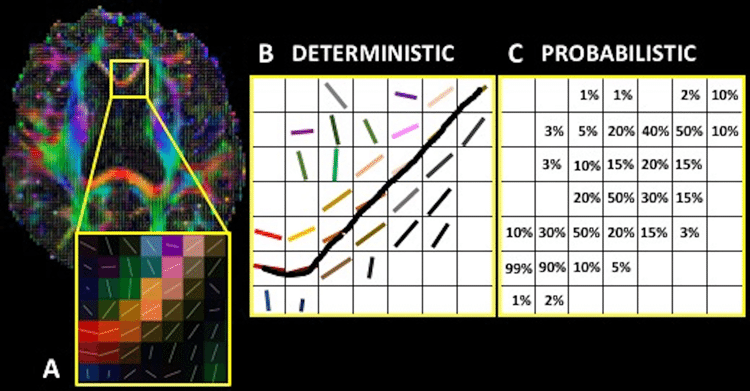
\includegraphics[width=0.7\textwidth]{images/A-Degree-of-anisotropy-B-Deterministic-fiber-tracking-the-fiber-path-across-voxels-is.png}
    \caption{Image from \cite{muller2018clinically} depicting different types of fiber tracking techniques. Red, green and blue indicate tracts runing along the x,y and z axis respectively. (a) Depicts deterministic tracking where the largest eigenvector determines the direction of progression along adjacent voxels. (b) Probabilistic tractograph is depicted, in each voxel a probability distribution function represents multiple possible diffusion directions.}
    \label{fig:tracking}
\end{figure}
Fiber tractography is a technique used to graphically construct  3 dimensional representations white matter pathways in the human brain. The technique uses the information about local fiber directions to trace streamlines that represent white matter tracts in the brain. It has become an important part of white matter disorder studies and has gained popularity because of its non-invasive nature. These advantages make it suitable for surgical targeting and planning \citep{romano2009pre}.

Tractography methods often use \gls{DTI} in order to delineate the streamlines along the white matter tracts by getting the information about their progression from one voxel to the next. This methodology relies on the assumption that the direction of maximum diffusion(in the diffusion tensor) aligns with the direction of the white matter fiber within the voxel. 

In deterministic tractography, the algorithm usually follows the direction of maximum diffusion from along the voxels by starting from a “seed” region. If the angle between two subsequent directions of maximum diffusion is less than predefined threshold then the algorithm proceeds tracking along the maximum diffusion direction of the second voxel and terminates when the condition is not met \cite{}. Several other conditions can also be imposed on the basis tracking technique on the basis of investigator specific techniques. The deterministic tractography does not take into account any random or systematic errors that arise during signal acquisition, recording and transmission.

Probabilistic tractography relies on estimation of a probability distribution function such as an fODF for the distribution of fiber orientations in each voxel. This helps to account for the possibility of crossing fibers and kissing fibers. The probability distribution functions and uncertainty are then used to build a path probability map corresponding to a seed point. Let's say N streamlines from a seed point a propagated by randomly using an orientation along the distribution functions. Between any to voxels 
\begin{align*}
P_{AB}= \frac{M}{N} & \textrm{ , probability that a curve starting at voxel A passes through voxel B} \\
M = & \textrm{ number of streamlines that go through B and A} \\
N = &\textrm{ total number of streamlines generated from A}
\end{align*}
Using this probability map the most probable fiber orientation can be determined. Multiple fiber orientations existing in a voxel, the one most compatible with the incoming trajectory is chosen \citep{behrens2003non}.
\subsection{Analyzing the brain as a graph}
\label{sec:braingraph}
The human brain is considered to be one of the most intricate biological systems. It has been well established that this complex system can be modelled as a network composed of various dynamically interacting elements. It can hence be well represented as a graph for computational analysis. The networks perspective has gained tractable attention in Neuroscience and given rise to an ever expanding field of Network Neuroscience. Brain networks can vary at scale (from molecular interactions to cognition. With different interactions at each level, graph theory finds its applications in this field \cite{sporns2018graph}. 

Graph theory can be defined as a branch of discrete mathematics that deals with the geometric analysis of graphs. Graph theory is useful in the analysis of biological networks since biological systems are dynamic and the interaction between the elements of the network gives rise to emergent properties. These properties can only be deciphered by comprehending the behavior with a systems approach. Graph theoretic methods can give comprehensive information about brain network topology, architecture, structure and function. This has given rise to the field of connectomics \citep{sporns2005human} for analysis of the structural and functional brain connectivity. The structural networks usually represent the anatomy of the brain and are temporally stable (ignoring effects of plasticity and development). On the other hand, the functional networks are temporally variable and dense.

Structural networks are preferred when trying to study the physical nature of the brain and it's anatomy, when trying to predict Neurological disorders and searching the biochemical basis and causal relationship various factors

\iffalse
A graph can be defined as mathematical representation of pairwise relationships between objects. A graph is said to consist of two basic elements i.e. nodes (representing the objects themselves) and edges (representing the relationships between the nodes). 
\fi


\subsection{Connectomics}
\label{sec:connectomics}
Connectomics is termed as the study of the brain's functional and structural networks. A connectome (in-vivo, retraced from imaging) is a dense network of brain connections, with a numerical value assigned to each network \citep{bassett2017network}. The connectome of brain can be seen as a circuit diagram with the neural connections analogous to wires and the cell bodies to electrical components.
Recently, connectomics has become the focus of major Neuroscience studies. Research in the field has expanded rapidly due to the increasing interest in understanding the brain as a dynamic system, and the belief that the connections in the brain are what give it its capabilities and functionality ( \cite{network_neuroscience_editorial}.

The first complete structural connectome to be mapped at the synaptic level was published in 1986,  belongs to the species C. elegans. It was reconstructed using electron micrographs of serial section and is a network that possess three hundred neurons and roughly seven thousand connections. It still took decades to claim the biological plausibility of all the connections in the reconstructed connectome\cite{elegans}, this leads to the fact that the connectome of the human brain cannot be mapped using the manual labour intensive methodology used by \cite{white1986structure}. Mapping the human brain manually hence seems implausible. The human brain contains roughly the same number of neurons as the stars in the Milky way galaxy and about $10^{15}$ inter neuronal connections called as synapses \citep{fornito2015connectomics}. This calls for the need to computationally determine brain connectivity from brain scans. Diffusion MRI can be used for sturcutral connectome construction while functional MRI is the preferred modality for functional connectome construction. The Human Connectome Project was launched in 2007 as the first large scale collaborative effort to create detailed maps of the brain (in-vivo) and to help better understand the fundamentals of human connectional anatomy.

\subsection{Structural Brain Connectivity}
%the term connectivity refers to several different and interrelated aspects of brain organization (Horwitz, 2003)
% is the anatomical connectivity in the brain
Structural brain connectivity refers to the arrangement of anatomical connections in the brain. A model of the brain's structural connectivity can be derived from whole brain tractography. In organisms such as humans with complex nervous systems, the structural brain connectivity can be visualized at different scales. It can be either at the level of synaptic connections (microscale), at the level of neuronal populations (meso-scale) or at macro scale in which fiber tracts run between different brain regions. At all these scales, the connectivity patterns of individuals from the same species exhibit different characteristics such as organization, topology and spatial extent \citep{Sporns:2007}.

Usually in Neuroimaging studies the connectivity is analyzed at the macroscopic scale, i.e. the running of the fibers between different brain regions.  From section \autoref{subsub:tractography} it can be inferred that the streamlines traced using the tractography algorithms represent the structural connections between different Regions of Interest(ROIs) of the brain seen as brain nodes. The connections are usually represented using bio-physical parameters such as mean FA (mean fractional anisotropy), number of streamlines between the two nodes and the length of the streamlines connecting the two nodes.


\section{Feature Selection Techniques}
\label{sec:feature_selection}
Neuroimaging data often suffers from the \textit{curse of dimensionality}. The sample size is often much smaller than the total number of features. Classifiers might be influenced by the increase in noise as the number of features increases. Dimensionality reduction and feature selection are often the techniques used for a meaningful reduction in features. However, most dimensionality reduction methods such as \gls{PCA} rely on transformations of the original data and this leads to a lack of interpretability. Due to this reason, it is important to consider feature selection methods where inference about which features the classifier learns can be made \citep{shi2018feature}. 

Feature selection methods can be grouped into three types; filter methods, wrapper methods and embedded methods. Filter methods are based on selecting features before running the classifier. Wrapper methods can be seen as a selection method \textit{on the fly} in which features are added or removed iteratively on the basis of classification performance. Embedded methods are those in which feature selection is embedded in the classifier. All three types of methods have been increasingly used in Neuroimaging studies, however filter methods remain advantageous due to interpretability considerations \citep{tohka2016comparison}.

\subsection{Filter methods}
\label{subsec:filtermethods}
Filters form one of the simplest methods for feature selection. They usually serve as a pre-processing step for the classification and are model independent. However, there is a caveat to use such techniques for classification studies. Each raw feature is considered independently and their cumulative effect is not taken into consideration for the classification. Some of the common techniques used to determine the feature importance is the use of coefficients such as the f-score and t-test which are widely used in Neuroimaging applications.

The f-score can be calculated as 
\begin{equation}
\label{eq:fscores}
    F = \frac{(\overline{x_{1}} - \overline{x})^2 + (\overline{x_{2}} - \overline{x})^2}
    {\frac{\sum_{i=1}^{n1}(x_{1,i} - \overline{x_{1}})^2}{n_{1} -1} + \frac{\sum_{i=1}^{n1}(x_{2,i} - \overline{x_{2}})^2}{n_{2} -1}}
\end{equation}
where $\overline{x}$ represents the average for all feature values, $\overline{x_{1}}$ the feature average for for the first class, $n_{1}$ represents the number of samples for the first class and other variables follow respectively.

A simple t-test can also be computed and then the features can be filtered based on the t-statistic or the p-value to test the significance of the differences between the feature values for two different groups. Based on \cite{inza2004filter}, the t statistic is calculated as:
\begin{equation}
    t = \frac{|\overline{x_1} - \overline{x_2}|}{\sqrt{0.5(\sigma_{1}^2 + \sigma_{2}^2)}}
\end{equation}
where $\sigma_{1}$ represents standard deviation for the feature values of the first group and $\sigma_{2}$ is the value for the second group. 
The features can be ranked on the basis of the p value of the t-test to obtain its statistical significance. Typically, values of $p<0.05$ are considered statistically significant \citep{colquhoun2017reproducibility}) and only then can the null hypothesis can be rejected with confidence. Numerical thresholds can also be applied for feature ranking if  such a methodology is suited to the nature of the problem. 

Based on a similar concept, the pearson correlation coefficient can be used to filter features if the target variables are continuous. The pearson correlation coefficient is defined as 
\begin{equation}
    \rho = \frac{\sum_{i=1}^{N} (x_{i} - \overline{x}) (y_{i} - \overline{y})}
    {\sqrt{\sum_{i=1}^{N} (x_{i}-\overline{x})^2 \sum_{i=1}^{N} (y_{i}-\overline{y}^2)}}
\end{equation}
where $y$ represents the target variable and $N$ represents the total number of data points. This takes the linear relationship between the feature values and the target variables into account.


\subsection{Maximum Weight Connected Subgraph}
\label{sec:MEWS}
\gls{MWCS} problem falls into the class of NP-hard problems. This method is widely used in biological network enrichment analysis \cite{DBLP:journals/corr/LobodaAS16}. One important application of this technique is to detect deferentially regulated pathways based on environmental or phenotypical changes \citep{althaus2014algorithms}). It can be extended to analyse brain networks to determine brain pathways which are correlated to a particular behavioral measurement/ physiological or epigenetic character. Since the number of connections are man, it is important to distinguish their properties etc, 

Consider an un-directed, connected graph $G = (V,E)$ with weighted nodes and edges. Let $V$ represents its set of vertices. $E$ the set of it's nodes, $w_e$ the weight of an edge $e$ and $w_v$ the weigh of a node $v$. Mathematically, the MWCS can be described as that subgraph  $\Tilde{G} = (\Tilde{V}, \Tilde{E})$ which maximizes the following function:
\begin{equation}
\label{eq:sumfun}
    \Omega(\Tilde{G}) = \sum_{v \in \Tilde{V}} w_v + \sum_{e \in \Tilde{E}} w_e \longrightarrow max
\end{equation}

The generalized MWCS can be converted into the Maximum Edge Weight Subgraph(MEWS) problem by either considering the weights of all the nodes in the  \autoref{eq:sumfun} as zero or equivalently constant valued so that the subgraph which maximizes the following constraint can be found.
\begin{equation}
    \label{eq:sumews}
    \Phi(\Tilde{G}) = \sum_{e \in \Tilde{E}} w_e \longrightarrow max
\end{equation}

According to the conceptual framework in \cite{DBLP:journals/corr/LobodaAS16}, such a problem is formulated using a Mixed Integer Programming (MIP) formulation. By using  a mixture of integral and binary variables, the maximal value of the objective function (\autoref{eq:sumfun}) can be optimally found using a set of constraints.

The first step of formulating such a problem is to represent a candidate optimal subgraph. The membership of nodes and vertices in the subgraph is represented using binary variables:
\begin{align}
    \label{eq:y_v}
    y_v = 1  \iff v \in V  \textrm{ and } v \in \Tilde{V} \\
    \label{eq:w_e}
    w_e =1  \iff e \in E  \textrm{  and }  e \in \Tilde{E}
\end{align}
Conceptually, an edge should be present in the subgraph only if both the end vertices are also present in the subgraph. In \autoref{eq:memberconstraint} this condition is represented as an inequality.
\begin{align}
    \label{eq:memberconstraint}
    w_e \leq y_v && \forall v \in V, e \in \delta_{v}
\end{align}
where $\delta_{v}$ represents the set of incoming edges on a node. Consider if $y_v = 0$, then $w_e$ has to be zero because an edge cannot be present without the node being present and if $y_v = 1$ then $w_e = 0$ or $w_e = 1$ because it is not necessary for an edge to be present if a node is present.

After the subgraph can be represented, it is important to establish the validity of any subgraph. A valid MWCS needs to be connected and maximise the function \autoref{eq:sumfun}. To establish the connectedness of the subgraph the concept of an arborescence needs to be introduced.

An arborescence is an acyclic directed graph in with a root node $v$, having exactly one path from $v$ to any other vertex $u$. The connectedness in a graph is defined as the existence of a simple path between any two nodes. So, for the valid connected subgraph each of it's traversal has to be a valid arborescence. The MWCS can be constructed in a bottom-up fashion by first determining the valid arboresnces and then combining them to form the optimal subgraph.

The traversal of any graph can be found by considering $S = (V,A)$ derived from $G=(V,E)$  where each undirected edge $(v,u)$ is replaced by two directed arcs $(u,v)$ and $(v,u)$. To ensure the connectedness of the subgraph (formed by combining arborescences) a non-linear formulation is needed where:
\begin{itemize}
     \setlength\itemsep{0.5em}
    \item Binary variable $x_a = 1$ iff $a \in A$ belongs to the arborescence.
    \item Binary variable $r_v = 1$ iff $v \in V$ is the root of the arborescence,
    \item Continuous variable $d_v = n$ if the length of the simple path from the root to the vertex v is n. The $d_v$ value can be arbitrary if the vertex v does not belong to the optimal solution
\end{itemize}
As pointed above, a valid arborescence corresponds to the traversal of the connected subgraph. Hence, the arborescence needs satisfy the following constraints, according to \cite{haouari2013enhanced}:
\begin{align}
    \label{eq:rv}
    \sum_{v \in V} r_v = 1\\
    \label{eq:dv}
    1 \leq d_v \leq n && \forall v \in V \\
    \label{eq:uvrv}
    \sum_{(u,v) \in A} x_{uv} + r_v = y_v && \forall v \in V\\
    \label{eq:fronba}
    x_{uv} + x_{vu} \leq w_e && \forall e =(v,u) \in A\\
    \label{eq:dvrv}
    d_v r_v = r_v\\
    \label{eq:dudv}
    d_u x_{vu} = (d_v + 1) x_{vu} && \forall e=(v, u) \in A
\end{align}
 \autoref{eq:rv} ensures that there is only one root of the arborescence. \autoref{eq:dv} limits the path length from the root vertex to any other vertex in the arborescence if it is present in the subgraph. With \autoref{eq:uvrv} it can be established if a vertex is a root then there are no incoming edges and that there is a maximum of one incoming edge on each node. The constraint in \autoref{eq:fronba} says that either the forward arc or the backward arc can be a part of the valid arborescence and not both. The last two constraints in \autoref{eq:dvrv}  and \autoref{eq:dudv} imposes that the length of the path to the root is always 1 and the distance of the nodes correspond to the direction of the edges.
It can be seen that  \autoref{eq:dvrv} and \autoref{eq:dudv} are non-linear. Combining the above equations the linearization is as follows:
\begin{align}
    \label{eq:dvlin}
    d_v + n r_v \leq n && \forall v \in V\\
    \label{eq:nuvlin}
    n + d_u - d_v \geq (n+1) x_{vu} && \forall (v,u) \in A\\
    \label{eq:dvdulin}
    n + d_v - d_u \geq (n-1) x_{vu} && \forall (v,u) \in A
\end{align}
\autoref{eq:dvlin} combines \autoref{eq:rv} and \autoref{eq:dv}. \autoref{eq:nuvlin} and \autoref{eq:dvdulin} can be justified with the fact that if a directed edge $(v.u)$ is present, then node $v$ is visited before node $u$ and $d_u - d_v = 1$. They hence represent the \autoref{eq:dudv}.
Any arbitrary node is considered to be the root of such an arborescence. The arborescence are then combined on the basis of the maximal edge and node weights to yield the final subgraph. 

\section{Classification}
\subsection{Support Vector Classifiers}
\begin{figure}
    \label{fig:svm}
    \centering
    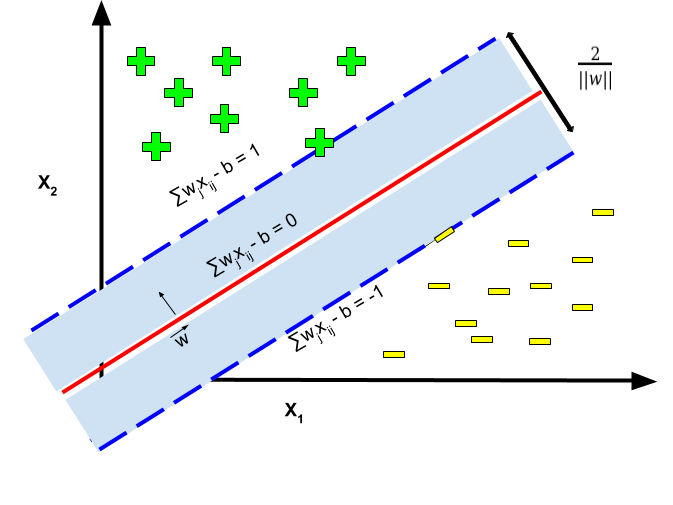
\includegraphics[width=0.75\textwidth]{images/SVM.png}
    \caption{Illustration of classification using support vector machines. The red line represents the decision boundary between the two classes.The algorithm maximizes the margin between the boundary for separate classes. The vectors lying on the hyperplanes depicted by the blue dashed lines are called as 'support vectors' and are the closest vectors to the decision boundary. Based on the values obtained by solving the L.H.S of the decision boundary for each data points, they are assigned to the corresponding classes.}
\end{figure}

Support Vector Classifiers (SVC) are classical machine learning algorithms based on Support Vector machines (SVMs). They are important since they have attained signifcant accuracy with different types of tasks such as a handwritten digits recognition, face detection in images, and text categorization \cite{burges1998a}. In Neuroimaging studies, SVCs are important for classification tasks since they are relatively robust to overfitting and more interpretable than Deep Learning classifiers.

In the simplest, binary case the mathematical formulation of the SVM is as follows. Consider each observation \textbf{$x_i$}, $i\in {1...n}$ to be a vector in the \textit{d-dimensional} feature space with a target label  $y_i\in {[-1,1]}$. The classifier needs to find a boundary that separates \textit{n} such points present in the presented data within a small margin of error.  It does so by trying to find an optimally separating hyperplane that efficiently divides the input data according to the target labels. In \autoref{fig:svm} the red line represents the optimally separating hyperplane that satisfies the equation
$ \sum w_i x_i - b = 0$
 It is maximally distant to the nearest point belonging to either class (also termed as the support vectors). The maximally separating hyperplane is found by satisfying the following constraints for each data point i. 
\begin{align}
    y_i(\sum_{j=1}^{d} w_{j} x_{ij}  + b)  - 1\geq 0 && \forall i \in {1...n}
\end{align}
Here, the weights represent the parameters the model learns in order to satisfy the above conditions by solving a Langrangian equation, the mathematics of which is beyond the scope of this text.  

In cases where the decision boundary is a non-linear function of the data the algorithm makes uses of what is commonly called as the 'kernel trick'. In this method the pairwise dot products of the individual $x_i$ are replaced by a non-linear transformation or kernel function. This expression then allows the algorithm to fit the maximum margin hyperplane in the transformed space. The decision boundary is linear in the transformed space and can be projected back to find the non-linear decision boundary in the original $d$ dimensional feature space. 
\subsection{Random Forest Classifiers}
\begin{figure}
    \centering
    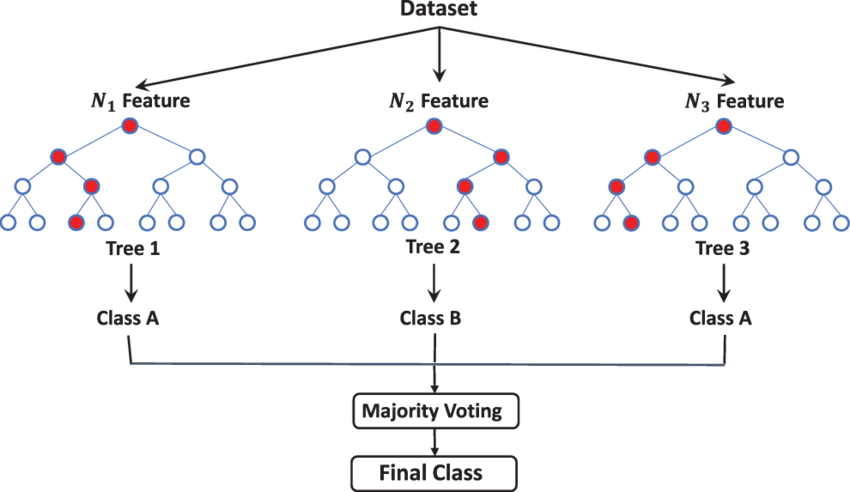
\includegraphics[width=0.8\textwidth]{images/Random_forest.png}
    \caption{Schematic explanation of Random Forest classifier from \cite{TAHMASEBI2020103619}. The different trees represent the decision trees constructed from the bootstrapped samples. Each tree is created on the basis of the most discriminatory features, $N_x$ for a particular bootstrapped sample. The final class of the samples in the dataset is decided on the basis of majority voting.}
    \label{fig:random_forests}
\end{figure}
\gls{RF2} Classifiers are based on the idea of bagging or bootstrap aggregation of decision trees \citep{hastie2009elements}. A decision tree is a way of recursively splitting the target variables on the basis of the rules set on the features. The name `Random Forest' comes from the fact that the algorithm builds a `forest' by aggregating a large number of de-correlated trees and averages them for building a classification. 

The Random Forest is built in the following manner. A number of runs is specified. First, a bootstrap sample is drawn from training data. On this bootstrapped data, one tree is grown by recursively splitting the tree tree until the minimum node size $n_{min}$ is reached. The steps for the recursive decision tree construction are:
\begin{itemize}
    \item Select $k$ variables randomly from the $p$ total variables
    \item Find the most predictive variable that has the most discriminatory split point
    \item Split the node into daughter nodes

\end{itemize}
This method is repeated to obtain a decision tree for each time a bootstrapped sample is obtained. The individual trees are the aggregated to make an ensemble on the basis of the ensemble vote of each tree. As it is evident from the \autoref{fig:random_forests}, the final classification of samples is based on the majority voting and hence a feature importance can be determined. The higher the position of a split in the random forest tree, the higher is its discriminatory power. Random forest classifiers are widely used in Neuroimaging studies due to the interpretability of features which can be obtained using the feature ranking in terms of the feature importance. 



\subsection{Multilayer Perceptron}
A \gls{MLP} is an Artificial Neural Network that is organized in the form of layers to mimic biological neural networks. The network consists of an input layer, an output layer as well as one or more hidden layers as shown in \autoref{fig:mlp}.b. Each layer consists of one or more artificial neurons (also called as perceptrons) which are connected to neurons of the subsequent layers. 

\begin{figure}
    \centering
    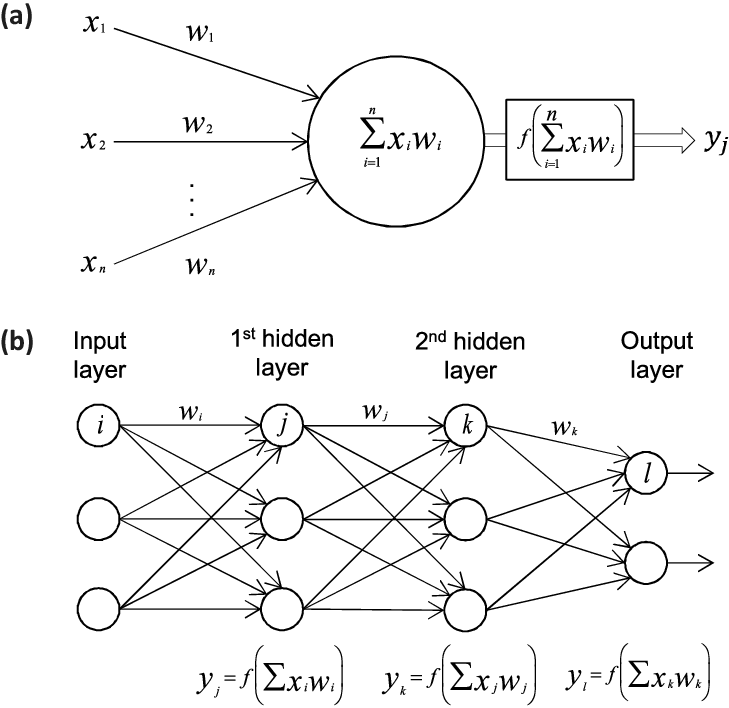
\includegraphics[width=0.5\textwidth]{images/tnn_ann.png}
    \caption{(a) Visualization of an artificial neuron from \cite{vieira2017using} depicting the output as a function of weighted sum of the inputs (\autoref{eq:op_neuron}) (b). The artificial neural network consisting of the input layer, hidden layers and the output layer.}
    \label{fig:mlp}
\end{figure}
The connections between the layers are feed-forward and uni-directional. The input layer serves as a buffer layer with no transformation of the input while in the other layers the neurons implement non-linear transfer functions on the weighted connections from the previous layer as shown in \autoref{fig:mlp}.a, the output $y$ from the neuron can be expressed as:
\begin{equation}
    \label{eq:op_neuron}
    y = g(\sum_{i=1}^{N} w_i x_i +b) 
\end{equation}
where $w_i$ represents the weighting of the inputs and b represents the bias for the neuron. Using the organizational structure, the neural network is able to learn complex transformations from the input data. In fact, it has been shown that an \gls{MLP} with just one hidden layer and a finite number of neurons is able to act as a universal function approximator \citep{universal_mlp}. Consider that we have an input vector in the N dimensional space and the output is needed in the M dimensional space. An \gls{MLP} (having non-linear transfer functional units) can implement any continuous mapping from the M dimensional space to the N dimensional space, with arbitrary accuracy. 

The network can be made `deep' by adding additional hidden layers. It is employed in Neuroimaging studies in use-cases where there is a requirement to eliminate the need for manual feature selection.


\end{document}
